\iffalse
% Mild cognitive impairment (MCI) is a transitional stage between age-related cognitive decline and Alzheimer’s disease (AD). For the effective treatment of AD, it would be important to identify MCI patients at high risk for conversion to AD. 
% The novel characteristics of the methods for learning the biomarkers are as follows: 1) We used a semi-supervised learning method (low density separation) for the construction of MRI biomarker as opposed to more typical supervised methods; 2)
% Alzheimer’s disease (AD), a common form of dementia, occurs most frequently in aged population.
% Mild cognitive impairment (MCI) is a transitional stage between age-related cognitive decline and AD, and the earliest clinically detectable stage of progression towards dementia or AD (Neuropathologic alterations in mild cognitive impairment: a review, Markesbery WR). 
% AD pathology has been therefore hypothesized to be detectable using neuroimaging techniques.(Neuropathologic alterations in mild cognitive impairment: a review, Markesbery WR)

% Only one study so far has applied deep learning algorithms, without a priori feature selection (considering gray matter [GM] volumes as input), to the prediction of AD development within 18 months in individuals with MCI using ADNI structural MRI scans (Suk et al., 2017, Deep ensemble learning of sparse regression models for brain disease diagnosis;).

To overcome the first limitation, many studies~\cite{brand2018joint,lu2018predicting} explored the temporal data structures of brain phenotypes over time. However, these models often formulate the longitudinal data as a tensor, which inevitably complicates the prediction problems. To ad- dress the second limitation of data inconsistency, most longitu- dinal models for AD studies (Wang et al., 2012b,a, 2017) only use the samples with complete temporal records and ignore the samples with fewer time points, which, however, may poten tially neglects substantially valuable information in the data. To solve this problem, data imputation methods (Xiang et al., 2014; Li et al., 2019) were used to generate missing records over AD progressions. Then the completed data are used for temporal regression analyses. However, missing data imputa- tion methods may introduce undesirable artifacts, which in turn can worsen the predictive power of the longitudinal models.
To take advantage of the full potential of longitudinal data with incomplete temporal inputs, in this paper we propose a novel method to learn an enriched biomarker representation to integrate the baseline records of the neuroimaging biomarkers of all the participants in a studied cohort and the dynamic measurements across the follow-up time points of the individuals in the same cohort. Instead solving the missing data problem using imputation, we tackle this challenging problem from a completely new and different perspective by learning a fixed-length vector. Second, we learn a local projection from the available follow-up neuroimaging records of every participant in the later couple of years to maintain the local data structures. Finally, a soft constraint is used to en- sure that the global and local projections are consistent. Using the learned projections, we can transform the medical records with inconsistent sizes in a neuroimaging dataset into a set of fixed-length vectors, which can be readily used by conventional machine learning models to predict cognitive outcomes for au- tomatic diagnosis of AD.
However there are crucial shortcomings in many current statistical models as they systematically perform independent learning at each point in time, missing the longitudinal changes characterized by temporal brain phenotypes.
Because AD is a chronic disease, First since AD is a chronic neurodegenerative disease, the progression of disease typically involves multiple consecutive neuroimaging records. Patient data are accumulated from different visits and form continuous patient supervision. The disease state at a certain point in time is not independent of the state at a previous point in time. 

In this study our main purpose is to classify the images which belong to two classes of very mild to mild AD and healthy subjects since this is the most crucial case for an efficient diagnosis of AD in order to prevent the patient’s condition from getting worse and more severe.

As a result, AD data are not only multi-modal but also time series. Consequently, considering AD multi-modal data as a time series is the intuitive solution for the AD progression problem. However, the vast majority of research does not consider this temporal/sequential nature of AD data.[alberdi2016early]
Liu et al. [liu2018joint] proposed a CNN-based model for joint AD classification and clinical score regression. The model is based on the fusion of MRI with three demographic features collected from baseline visits only. Most of the Alzheimer’s DL models are based on the CNN and single (baseline) MRI scans [Fusion of deep learning models of MRI scans, Mini–Mental State Examination, and logical memory test enhances diagnosis of mild cognitive impairment]. These models are less accurate, less sufficient, and not medically acceptable, because a medical expert usually studies the longitudinal multi-modal patient data before making progression decisions [ding2018hybrid].
The main contributions of this work can be summarized as follows.
- We propose an advanced multi-modal multitask DL architecture for detecting AD progression. The framework leverages the patient’s time series data to jointly predict multiple variables from multiple sources. The resulting comprehensive system is medically intuitive, more stable, and more accurate than existing state-of-the-art studies.

% To overcome the first limitation, many studies~\cite{brand2018joint,lu2018predicting} explored the temporal data structures of brain phenotypes over time. However, these models often formulate the longitudinal data as a tensor, which inevitably complicates the prediction problems. To address the second limitation of data inconsistency, most longitudinal models for AD studies (Wang et al., 2012b,a, 2017) only use the samples with complete temporal records and ignore the samples with fewer time points, which, however, may poten tially neglects substantially valuable information in the data. 
% To solve this problem, data imputation methods (Xiang et al., 2014; Li et al., 2019) were used to generate missing records over AD progressions. Then the completed data are used for temporal regression analyses. However, missing data imputation methods may introduce undesirable artifacts, which in turn can worsen the predictive power of the longitudinal models.
% Instead solving the missing data problem using imputation, we tackle this challenging problem from a completely new and different perspective by learning a fixed-length vector. First, our model learns a global projection from the baseline records of the biomarkers of all the participants to preserve as much information as possible. 

% On the other hand, besides AD and HC subjects, we often have MR brain images available from other related subjects such as those with mild cognitive impairment (MCI), a prodromal stage of AD, or possibly the unrelated subjects whose cognitive statuses may be not known.
% Semi-supervised classification approaches are specifically designed to handle cases where only part of the data is labeled.
% In contrast, semi-supervised SVM considers both labeled and unlabeled data, and may be more appropriate in the scenario where the labeled population does not entirely reflect the structure of the data.
% Commonly used supervised pattern recognition methodology may not be the most suitable approach to deriving image-based biomarkers in such cases, as it relies on the availability of categorically labeled data (e.g., patients and controls)

\fi

\section{Introduction}
% Why our model is good? : (1) Semi-supervised learning -> Our model can learn from labeled/unlabeled samples BOTH. (2) Learn temporal trends from the time series with missing records (MRI imagings are captured inconsistently (the number of records/the time points of records are different) from the participants). (3) Combine the multi-modal (genotypic modality (SNPs, static) + phenotypic (neuroimagings, dynamic) modality) data with two Autoencoders: one for static, another for time series.
% Find the related works with the lack of above advantages of our model.
Alzheimer's Disease (AD) is a chronic neurodegenerative disease that impairs patients' thinking, memory, and behavior. More than 30 million people worldwide suffer from AD, and with the increase in life expectancy this figure is projected to triple by 2050~\cite{barnes2011projected}. AD typically advances from a pre-clinical level to mild cognitive impairment (MCI) and eventually to AD, along a time scale. Early identification of at-risk individuals is crucial in slowing disease progression and many researchers have dedicated their efforts to identify AD relevant biomarkers and develop a computer-aided system to accurately predict AD onset.
Neuroimaging has sparked interest among researchers seeking to characterize AD progression due to it's widespread availability that takes advantage of high spatial resolution and good contrast between different soft tissues~\cite{stonnington2010predicting,wang2012phenotype,brand2018joint}.
However, there are a few limitations to the existing neuroimaging analysis models. 
% First, many of them routinely perform standard regression or classification at each individual time point separately, and do not take advantage of the longitudinal structure among temporal brain phenotypes.
First, since AD is a progressive neurodegenerative disorder, many longitudinal models~\cite{brand2018joint,wang2012high,wang2016prediction,wang2017longitudinal} have been proposed to explore the temporal relationships among neuroimaging records. However, they only consider the order of records, not their time intervals between the records.
% \cite{brand2018joint,wang2012high,wang2016prediction,wang2017longitudinal}

% Second, measurements of neuroimaging biomarkers are often missing at certain time points for some participants. This is because higher mortality rate and cognitive disability discourage older adults from staying in studies that require multiple visits, making it difficult to consistently sample medical scans from a large participant pool. Although the missing data issue is prevalent in most medical datasets, many studies assume feature-complete data or simply remove samples with missing data~\cite{stonnington2010predicting,liu2018joint}, harming the integrity of the dataset. 
% % \cite{stonnington2010predicting,sukkar2012disease,lei2017relational,liu2018joint}
% Recently, several data imputation methods~\cite{xiang2014bi,li2019multi} have been proposed to generate missing records of longitudinal AD measures, however these data imputation methods can introduce undesirable bias that degrades a model's predictive power.

Second, diagnosing AD involves a number of medical tests, leading to large collections of heterogeneous, multivariate results of dynamic and static data.
% Because of the heterogeneous composition of medical examinations, it can be challenging and tedious to manually compare, visualize and evaluate these data; thus an efficient approach to predicting the brain's condition accurately through classifying magnetic resonance imaging (MRI) images is highly advantageous and yet quite difficult.
As a result, AD patients are characterized by heterogeneous multi-modalities which does help to identify and differentiate the subtle shifts in disease progression and promote accurate diagnoses. 
% \cite{qiu2018fusion,cui2011identification}
However, records of dynamic data are often missing at certain time points for some participants. This is because higher mortality rate and cognitive disability discourage older adults from staying in studies that require multiple visits, making it difficult to consistently sample medical scans from a large participant pool.
As a result, integrating multi-modal data is challenging because the dynamic data is represented by a matrix of varying size and the static data is represented by the fixed-length vector. Current longitudinal methods~\cite{wang2016prediction,langkvist2014review,srivastava2015unsupervised} often do not combine the complementary information from different modalities to improve diagnostic precision.

Third, the biomarkers of AD can be obtained even if the diagnoses for some participants is missing, but collecting the labeled data is time consuming and costly. Recent recurrent neural networks (RNNs)~\cite{medsker2001recurrent}, especially Long Short Term Memory (LSTM)~\cite{schmidhuber1997long}, have been successfully applied in longitudinal dataset analysis due to their flexibility to handle missing data and ability to learn long-term dependencies. Although effective, they are supervised learning~\cite{vieira2017using,hong2019predicting,tabarestani2019longitudinal} models which cannot learn from unlabeled samples. In the application of LSTM to unsupervised learning, the previous studies~\cite{langkvist2014review,srivastava2015unsupervised} learn the representation of dynamic data in a lower dimensional space. The proper representation of dynamic data is crucial because dynamic data usually contains noises and redundant information from the large number of features and records~\cite{tuncel2018autoregressive,langkvist2014review}. While these models do utilize unlabeled samples, they encode the dynamic data into another longitudinal representation which is difficult to integrate with the static data. In addition, they often do not utilize the labeled samples, which is a missed opportunity to improve the representation learning for better predictions.

% Under these circumstances, a semi-supervised approach is more appropriate, as it can learn from both labeled and unlabeled data.
% In a semi-supervised approach, the unlabeled samples are also used in the learning process in addition to the labeled samples.
% In the recent years, there have been a number of deep learning applications to classify the AD progression with Alzheimer's Disease Neuroimaging Initiative (ADNI) dataset~\cite{vieira2017using}, but many of them are supervised or unsupervised learning approaches which are not suitable for the cases where only part of the data are labeled.

To take full advantage of heterogeneous longitudinal data, we propose a novel semi-supervised learning method to learn an enriched biomarker representation for each participant in a studied cohort. The proposed model consists of two autoencoders~\cite{kramer1991nonlinear}; The deep neural network autoencoder and long short-term memory (LSTM) autoencoder each learn the vectorial representation from static genetic data and dynamic phenotypic data. The enriched representation of dynamic data is in a fixed-length vector format, which can be readily integrated with the enriched representation of static data as illustrated in Fig.~\ref{fig: overview}.
% In this research, given multi-modal longitudinal biomarkers with one or more time points, we aim to predict clinical diagnosis.
% In this paper, we propose a novel deep learning approach to learn a abstract vectorial representation of neuroimaging modalities.
\begin{figure}[h]
    \centering
    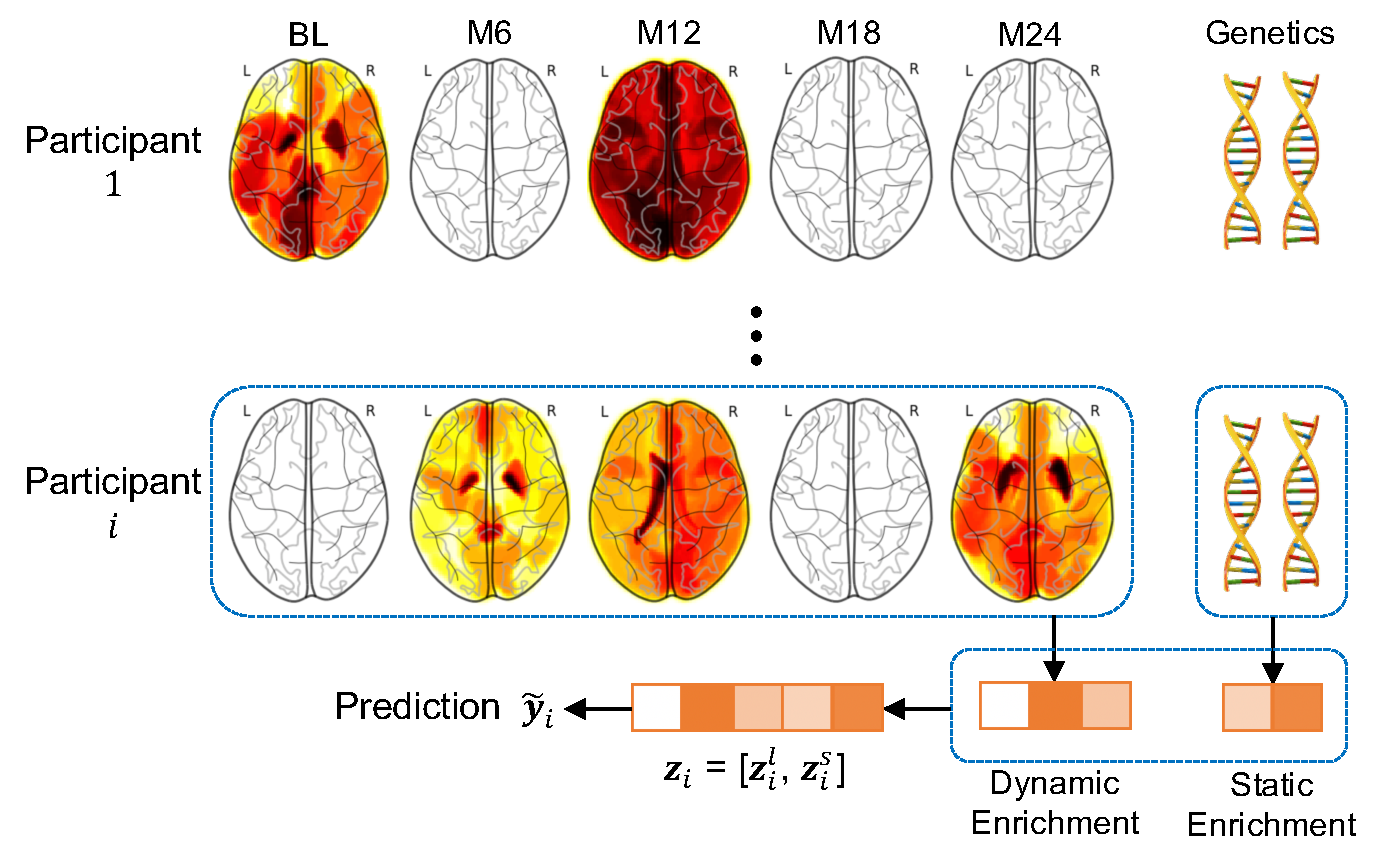
\includegraphics[width=0.87\textwidth]{images/overview.pdf}
    \caption{Illustration of the proposed model to integrate dynamic and static data via enrichment. The blank brain plots denote the missing scans of a participant. 
    % The dynamic enrichment summarizes the longitudinal records with missing data into a fixed-length vectorial representation.
    } \label{fig: overview}
\end{figure}
% The proposed approach has the following benefits compared to the existing models:
% (1) The LSTM autoencoder learns the new representation of dynamic data in a fixed-length vector format, which can be easily integrated with the static data.
% (2) We learn the representations of dynamic data incrementally, considering the uneven time intervals between the records.
% (3) Our model fully utilizes the available labels of samples.
% (4) We do not rely on the imputation or discarding of samples to handle missing data.
% (1) LSTM autoencoder explicitly utilizes the time stamp of each longitudinal record to uncover the temporal relation between the records,
% (3) the proposed model integrates the multiple modalities, such as longitudinal (dynamic) phenotypic data, static genetic data and demographic information,
% ~\cite{tian2018deep}

%  We identify the AD relevant biomarkers through the perturbation based feature identification.
% We outline the proposed model in Fig~\ref{fig: overview}.
% Reduce references criticizing the previous works.
